\documentclass[a4paper,14pt]{extarticle}

\usepackage[left=30mm, right=10mm, top=20mm, bottom=20mm]{geometry}

\usepackage[T2A]{fontenc}
\usepackage[utf8]{inputenc}
\usepackage[russian]{babel}
\usepackage{tempora}
\usepackage{type1cm}
\usepackage{indentfirst}

\usepackage{minted}
\usepackage{xcolor}

\usepackage{siunitx}
\usepackage{booktabs}
\usepackage{multirow}


\usepackage{csquotes}
\usepackage[
    parentracker=true,
    backend=biber,
    style=gost-numeric,
    sorting=nty
]{biblatex}

\usepackage[nodisplayskipstretch]{setspace}
\usepackage[none]{hyphenat}
\usepackage{fancyhdr}
\usepackage{titlesec}
\usepackage{tocloft}

\usepackage{amssymb}
\usepackage{amsmath}
\usepackage{tikz}
\usepackage{pgfplots}
\usepackage{graphicx}
\usepackage{caption}
\usepackage{subcaption}
\usepackage[hidelinks]{hyperref}
\usepackage[russian]{cleveref}
\usepackage{bookmark}

\pgfplotsset{compat=1.18}

\onehalfspacing
\sloppy

\pagestyle{fancy}
\fancyhf{}
\fancyfoot[R]{\thepage}
\renewcommand{\headrulewidth}{0pt}

\definecolor{codebg}{rgb}{0.12,0.12,0.14}
\definecolor{codeframe}{rgb}{0.40,0.40,0.45}
\definecolor{keywordcolor}{rgb}{0.45,0.65,1.0}
\definecolor{stringcolor}{rgb}{1.0,0.55,0.45}
\definecolor{commentcolor}{rgb}{0.55,0.75,0.60}
\definecolor{textcolor}{rgb}{0.90,0.90,0.90}

\renewcommand{\theFancyVerbLine}{
	\sffamily\small\color{black}\arabic{FancyVerbLine}
}

\setminted{
    bgcolor=codebg,
	fillcolor=codebg,
	framesep=1em,
	frame=single,
    rulecolor=\color{codeframe},
    fontsize=\normalsize,
    baselinestretch=1.1,
    linenos,
    numbersep=6pt,
    tabsize=4,
    breaklines,
    breakbytoken,
	breaksymbolleft={},
    autogobble,
    showspaces=false,
    showtabs=false,
}

\usemintedstyle{lightbulb}
\setmintedinline{
    bgcolor=codebg
}

\makeatletter
\setlength{\@fptop}{0pt}
\setlength{\@fpsep}{8pt}
\setlength{\@fpbot}{0pt plus 1fil}
\makeatother

\newcommand{\circledequals}{\mathbin{\tikz \node[draw,circle,inner sep=1pt] {$=$};}}

\begin{document}
    \begin{titlepage}
		\centering
		
		
\includegraphics{images/FEFU-logo.jpg}\\
		МИНИСТЕРСТВО ОБРАЗОВАНИЯ И НАУКИ РОССИЙСКОЙ ФЕДЕРАЦИИ\\
		Федеральное государственное автономное образовательное учреждение высшего образования\\
		\textbf{«Дальневосточный федеральный университет»}

		\rule{\linewidth}{0.8mm}\\[0.3cm]
		
		\textbf{ИНСТИТУТ МАТЕМАТИКИ И КОМПЬЮТЕРНЫХ ТЕХНОЛОГИЙ}\\
		\textbf{Кафедра математического и компьютерного моделирования}\\
		\vspace*{0.9cm}
		
		Кулахсзян Сергей Грайрович\\
        \vspace*{0.3cm}

		ЛАБОРАТОРНАЯ РАБОТА № 4 \\
        ЗАДАЧА № 22 \\
		\vspace*{0.5cm}

		\textbf{Задачи на смеси}\\
		\vspace*{0.5cm}

		Направление подготовки 02.03.01сцт Сквозные цифровые технологии,\\ 
        бакалавриатская программа «Математика и компьютерные науки»\\ 
        Очной формы обучения\\
		\vspace{1.5cm}
		
		\vfill
		\centering
		г. Владивосток\\
		2026
	\end{titlepage}

    \tableofcontents
    \thispagestyle{empty}

	\newpage
    \pagenumbering{arabic}
    \setcounter{page}{3}
    \section{Постановка задачи}
    В баке находится 150 л морской воды, содержащей 4 \% соли. 
    В бак подаётся пресная вода со скоростью 4 л/мин.
    Полученная смесь перемешивается и вытекает со скоростью 6 л/мин.
    
    Какой станет концентрация соли через час?

    \section{Математическое моделирование}
    Перед построением модели сделаем допущение: перемешивание происходит настолько интенсивно, что в любой момент времени смесь можно считать однородной.

    $V(t)$ -- объём соли (в литрах) в баке в момент времени $t$ (в минутах).
    Так как каждую минут в бак втекает 4 л, а вытекает 6 л, то к моменту времени $t$ в баке будет $(150 -2t)$ л жидкости.
    Из этого следует, что концентрация соли составит: 
    \begin{equation}
        \displaystyle \delta(t) = \frac{V(t)}{150 - 2t} \text{ \%}.
    \end{equation}

    За промежуток $\Delta t$ из бака выльется $6 \Delta t$ л смеси.
    Если предположить, что концентрация соли в этом промежутке времени не изменяется, то смесь содержит $\displaystyle \frac{V(t) \cdot 3\Delta t}{75 - t}$ л соли.

    Но  концентрация соли всё же уменьшается, поэтому верно неравенство:
    \begin{equation} \label{inequality}
        \displaystyle \frac{V(t + \Delta t) \cdot 3\Delta t}{75 - t} < V(t) - V(t + \Delta t) < \frac{V(t) \cdot 3\Delta t}{75 - t}.
    \end{equation}

    Деля (\ref{inequality}) на $\Delta t$ и устремляя $\Delta t$ к 0, получаем дифференциальное уравнение:
    \begin{equation*}
        \displaystyle -V' = \frac{3V}{75 - t}.
    \end{equation*}
    Добавляя начальное условие в момент времени $t_0$ и с начальным объёмом соли $V_0$, получаем математическую модель:
    \begin{equation*}
        \begin{cases}
            \displaystyle V' = \frac{3V}{t - 75} \\
            V(t_0) = V_0
        \end{cases}.
    \end{equation*}

    Так как в начальный момент времени концентрация соли составляла 4 \% от 150 л, то:
    \begin{equation} \label{model}
        \begin{cases}
            \displaystyle V' = \frac{3V}{t - 75} \\
            V(0) = 6
        \end{cases}.
    \end{equation}

    \section{Аналитическое решение}
    Уравнение (\ref{model}) имеет следующее решение: \\
    $\displaystyle
    \frac{dV}{V} = \frac{3dt}{t - 75} \\
    \ln V = 3\ln |t - 75| + \ln c \\
    V(t) = c|t - 75|^3 \\
    V(0) = 75^3 c = 6 \Rightarrow c = \frac{6}{75^3} \\
    V(t) = 6 \left| \frac{t}{75} - 1 \right|^3 \\
    V(60) = \frac{6}{5^3} \text{ л} \\
    \delta(60) = \frac{6}{5^3 \cdot (150 - 120)} = 5^{-4} = 0.0016 = 0.16 \%. \\
    $
    Тогда получаем, что концентрация соли через час составит 0.16 \%.

    \section{Численное решение}
    Для численного решения уравнений был применён метод Рунге-Кутта 4-го порядка, который имеет погрешность $O(h^4)$: \\
    $\displaystyle
    V_{i + 1} = V_i + \frac{h}{6} (k_1 + 2k_2 + 2k_3 + k_4), \\
    k_1 = f(t_i, V_i), \\
    k_2 = f \left( t_i + \frac{h}{2}, V_i + \frac{h}{2} k_1 \right), \\
    k_3 = f \left( t_i + \frac{h}{2}, V_i + \frac{h}{2} k_2 \right), \\
    k_4 = f(t_i + h, V_i + h k_3).
    $

    Вычисление было произведено на отрезке $[1; 10]$ при значениях $N = 10; 100; 1000$.
    В ходе выполнения были получены следующие результаты представленные на графиках:

    \begin{figure}[H]
        \centering
        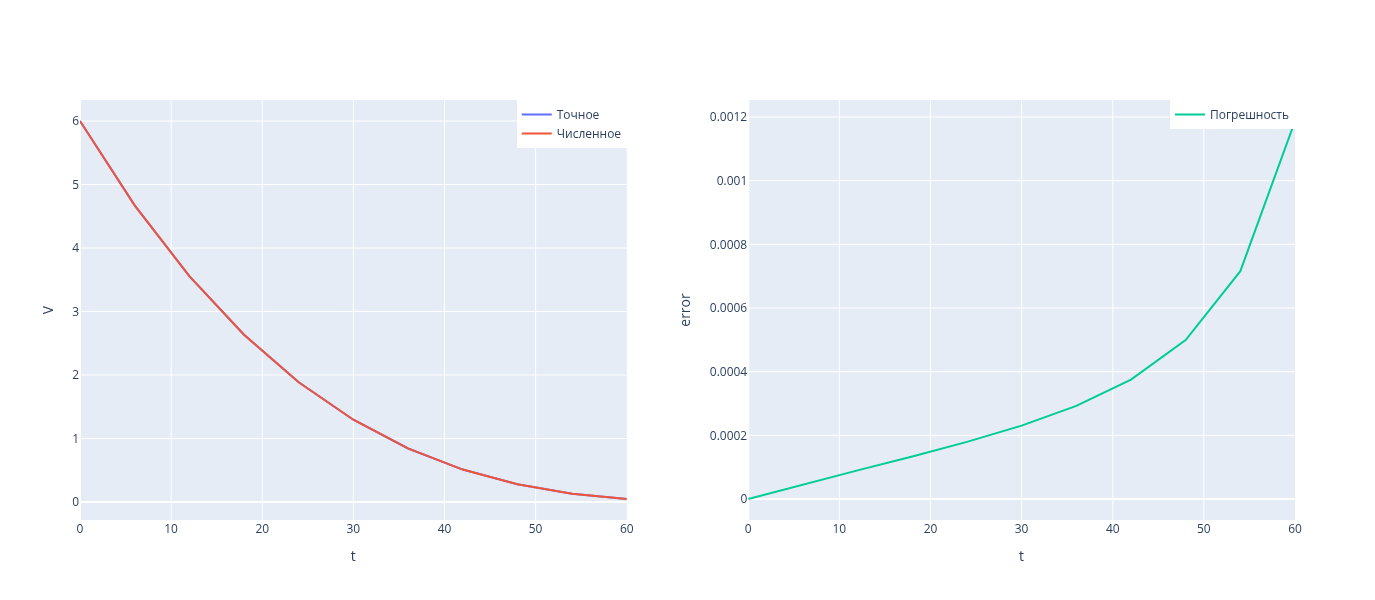
\includegraphics[width=\textwidth]{images/10.png}
        \caption{Тестирование решения при $N = 10$}
        \label{n_10}
    \end{figure}

    \begin{figure}[H]
        \centering
        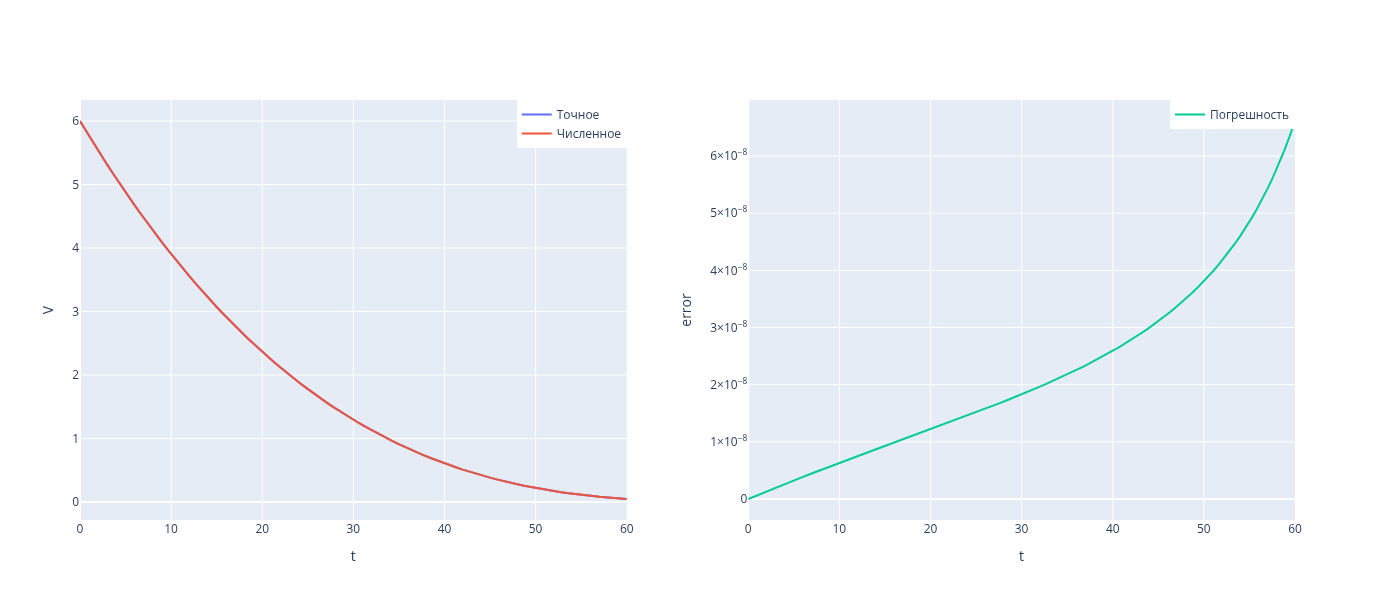
\includegraphics[width=\textwidth]{images/100.png}
        \caption{Тестирование решения при $N = 100$}
        \label{n_100}
    \end{figure}

    \begin{figure}[H]
        \centering
        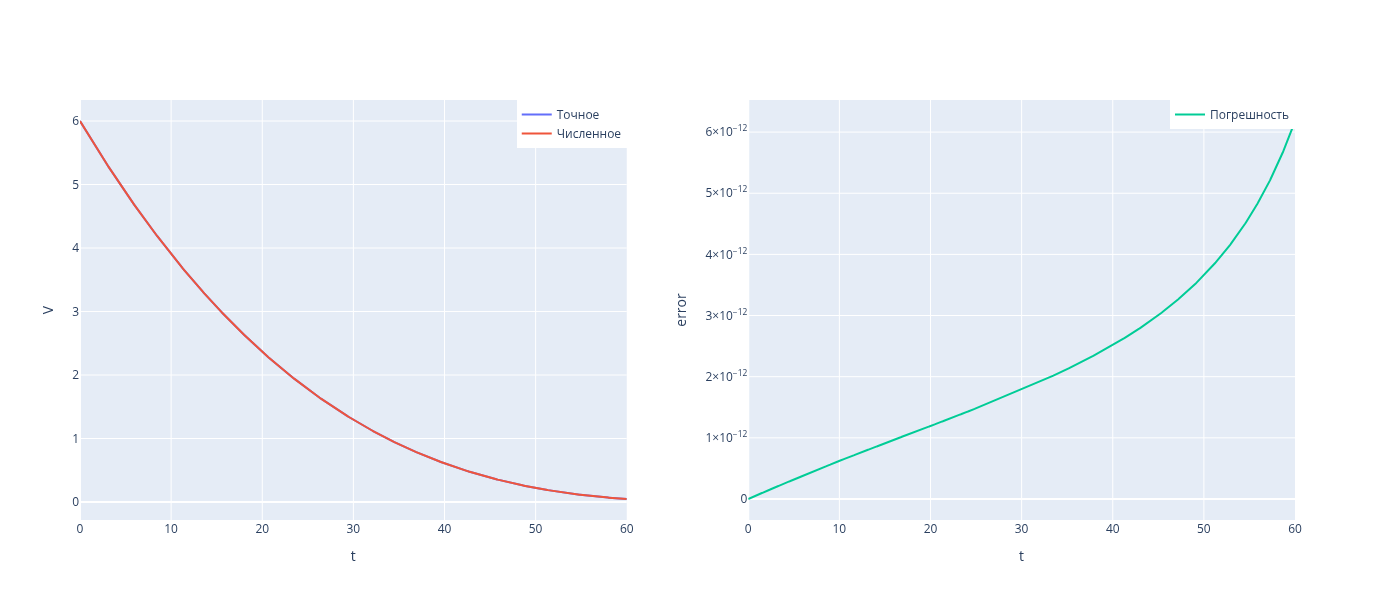
\includegraphics[width=\textwidth]{images/1000.png}
        \caption{Тестирование решения при $N = 1000$}
        \label{n_1000}
    \end{figure}

    \section{Заключение}
    В ходе лабораторной работы была рассмотрена и решена задача на реактивное движение. 
    Сравнение численных и аналитических решений, приведённое на графиках (\cref{n_10}, \cref{n_100}, \cref{n_1000}), показало, что при увеличении числа узлов сетки численное решение всё точнее приближается к аналитическому.
    Ответ был получен 0.16 \%.
\end{document}